\documentclass{report}
\usepackage[
  inner	=	3.0cm, % Margen interior
  outer	=	2.5cm, % Margen exterior
  top	=	2.5cm, % Margen superior
  bottom=	2.5cm, % Margen inferior
  includeheadfoot, % Incluye cabecera y pie de página en los márgenes
]{geometry}
% Valor de interlineado
\renewcommand{\baselinestretch}{1.0} % 1 línea de interlineado

% Paquetes imprescindibles para la portada
\usepackage{fontspec} % Para poder importar las fuentes
\usepackage{textpos} % Para posicionar bloques de texto
\usepackage{graphicx} % Para cargar imágenes
\graphicspath{{./Imagenes}}
\usepackage{setspace} % Para modificar los espacios arriba y abajo
%Otros paquetes
\usepackage[spanish]{babel}
\usepackage{fancyhdr}
\usepackage{hyperref} 
\hypersetup{
    colorlinks=true,
    urlcolor=blue,
    }
\usepackage{mathtools}
\usepackage{amssymb}
\usepackage{amsmath}
\usepackage{booktabs}
\usepackage{multirow}
\usepackage{caption}
\usepackage{mathtools, nccmath}

\usepackage[T1]{fontenc}
\usepackage{tocloft}
\DeclarePairedDelimiter{\nint}\lfloor\rceil
\captionsetup[table]{name=Tabla}
\DeclarePairedDelimiter\abs{\lvert}{\rvert}%
\DeclarePairedDelimiter\norm{\lVert}{\rVert}%

\usepackage{color}
\usepackage{colortbl}
\usepackage{tcolorbox}
\usepackage{xcolor}
\usepackage{listings}
\usepackage{float}


%%%%%%%%%%%%%%%%%%%%%%%%
    %CODE CONF
%%%%%%%%%%%%%%%%%%%%%%%%
\definecolor{Naranjastring}{HTML}{FF5733}
\definecolor{k3}{HTML}{27A48A}
\definecolor{codeorange}{HTML}{EE7623}
\definecolor{codegray}{rgb}{0.5,0.5,0.5}
\definecolor{codepurple}{rgb}{0.58,0,0.82}
\definecolor{backcolour}{HTML}{003B4D}
\definecolor{funccolor}{HTML}{C1531B}
\definecolor{color-lang}{HTML}{C1C5C8}
\definecolor{colorvar}{HTML}{7398AD}
\definecolor{green--}{HTML}{A0CA92}
%---------------------- C ----------------------- %

\lstdefinestyle{myCstyle}{
  backgroundcolor=\color{backcolour},   
  commentstyle=\color{codeorange},
  keywordstyle=\color{codeorange},
  numberstyle=\tiny\color{codegray},
  stringstyle=\color{green--},
  basicstyle=\ttfamily\footnotesize\linespread{0cm}\color{color-lang},
  breakatwhitespace=false,                         
  captionpos=b,                    
  keepspaces=false,                                                                   
  showstringspaces=false,
  showtabs=false,                  
  tabsize=2,
  inputpath = código,
  postbreak=\mbox{\textcolor{red}{$\hookrightarrow$}\space},
  breaklines = false,
  keywordstyle=[2]\color{codepurple},
  keywordstyle=[3]\color{funccolor},
  keywordstyle=[4]\color{colorvar},
  keywordstyle=[5]\color{Naranjastring},
  keywords=[2]{f},
  keywords=[5]{STLIB, LinearSensor},
  keywords=[4]{value, slope, offset, pressure_1, Board, PF11},
  keywords=[3]{main, start, read, update,printf},
  morekeywords = {_delay_ms, sei, ISR, uint8_t, LinearSensor, uint16_t, STLIB, }
  %firstnumber=(auto|last|<number>) para comenzar el conteo de lineas de listing con otro numero. Auto empieza por 1, last, continua la cuenta del listing anterior, number es un numero cualquiera.
}


% set listings
\lstset{%
    basicstyle=\footnotesize\ttfamily,
%   captionpos=t,
    framesep=5em,
    language = C++, style=myCstyle
}

% define backgroundcolor
\definecolor{bggray}{HTML}{003B4D}

% add frame environment
\usepackage[%
    framemethod=tikz,
    skipbelow=\topskip,
    skipabove=\topskip
]{mdframed}
\mdfsetup{%
    leftmargin=0pt,
    rightmargin=0pt,
    backgroundcolor=bggray,
    middlelinecolor=black,
    roundcorner=7
}

\usepackage{etoolbox}% >= v2.1 2011-01-03
\BeforeBeginEnvironment{lstlisting}{\begin{mdframed}\vspace{-0.4em}}
\AfterEndEnvironment{lstlisting}{\end{mdframed}}

% needed for \lstcapt
\def\ifempty#1{\def\temparg{#1}\ifx\temparg\empty}

% make new caption command for listings
\usepackage{caption}
\newcommand{\lstcapt}[2][]{%
    \ifempty{#1}%
        \captionof{lstlisting}{#2}%
    \else%
        \captionof{lstlisting}[#1]{#2}%
    \fi%
    \vspace{0.75\baselineskip}%
}

%%%%%%%%%%%%%%%%%%%%%%%%
        %CODE CONF end%
%%%%%%%%%%%%%%%%%%%%%%%%

\newcommand{\Universidad}{Universitat Politècnica de València}
\newcommand{\LogoUniversidad}{LogoUPV}
\newcommand{\Facultad}{Escola Tècnica Superior d'Enginyeria Informàtica}
\newcommand{\LogoFacultad}{Logo_etsinf}
\newcommand{\Titulacion}{Grado en Ingeniería Informática}
\newcommand{\titulo}{\scshape ST-LIB: librería de abstracción de microcontroladores STM32}
% Tipo de trabajo
\newcommand{\tipotrabajo}{Trabajo de fin de grado}
% Datos del autor
\newcommand{\miNombre}{Ricardo Chust Fides}
\newcommand{\miTutor}{ Vicente Atienza}
\newcommand{\colaboradores}{ Daniel González, Stefan Costea, Alejandro Gonzalvo, Pablo González}

% Ubicación
\newcommand{\miUbicacion}{València}
\renewcommand{\thetable}{\arabic{table}}
\renewcommand\spanishtablename{Tabla}
\renewcommand\spanishfigurename{Diagrama}

\begin{document}
\setcounter{secnumdepth}{3}

%%%%%%%%%%%%%%%%%%%%%%%%%%%%%%%%%%%%%%%%%%%%%%%%%%%%%%%%%%%%%%%%%%%%%%%%
% Plantilla TFG/TFM
% Realizado por: Jose Manuel Requena Plens
% Contacto: info@jmrplens.com / Telegram:@jmrplens
%%%%%%%%%%%%%%%%%%%%%%%%%%%%%%%%%%%%%%%%%%%%%%%%%%%%%%%%%%%%%%%%%%%%%%%%

% esta plantilla ha sido ligeramente modificada por Ricardo Chust Fides para
%habilitar CoAutores y Tutor en ella

% Fuentes
\newfontfamily\ArialMT{ArialMT}[Path=./fuentes/] 
\newfontfamily\ArialBoldMT{Arial-BoldMT}[Path=./fuentes/] 
\newfontfamily\ArialBoldItalicMT{Arial-BoldItalicMT}[Path=./fuentes/] 

\begin{titlepage}

% Márgenes de esta pagina modificados
\newgeometry{ignoreall,top=2.5cm,bottom=1cm,outer=2.5cm,inner=2.5cm}

% Pagina sin estilo
\thispagestyle{empty}

%%%%%%%%%%%%%%%%%%%%%%%%%%%%%%%%%%%%%%%%%%
% Universidad, facultad y titulación
\noindent\begin{minipage}{\textwidth}
\centering
% Universidad
 {\ArialMT\fontsize{20pt}{25pt}
 {\addfontfeature{LetterSpace=1.0}
 {\MakeUppercase\Universidad}}}\\[0.5cm]
% Facultad
 {\ArialBoldMT\fontsize{14pt}{17pt}
 {\addfontfeature{LetterSpace=10.0}{
 \MakeUppercase\Facultad}}}\\[0.42cm] 
% Titulación
 {\ArialBoldMT\fontsize{13pt}{16pt}
 {\addfontfeature{LetterSpace=16.0}{
 \Titulacion}}}
\noindent\rule[-0.22cm]{\textwidth}{5pt} % Linea
\end{minipage}

% Relleno hasta logotipos
\vfill

%%%%%%%%%%%%%%%%%%%%%%%%%%%%%%%%%%%%%%%%%%
% Logotipos
% Universidad
\begin{textblock*}{5cm}(0.80cm,-6.52cm)% Ancho - Pos X,PosY
	 \includegraphics[width=3.5cm]{\LogoUniversidad}
\end{textblock*}
% Facultad
\begin{textblock*}{12cm}(5.0cm,-5.82cm)% Ancho - Pos X,PosY
	 \includegraphics[width=11cm]{\LogoFacultad}
\end{textblock*}

% Relleno hasta el título
\vfill

%%%%%%%%%%%%%%%%%%%%%%%%%%%%%%%%%%%%%%%%%%
% Título
\begin{textblock*}{\textwidth}(0cm,-6.1cm)% Ancho - Pos X,PosY
\noindent
\begin{minipage}{\textwidth}
\begin{spacing}{2.1}
 \centering
  {\fontsize{25pt}{30pt} \fontfamily{cmr}\selectfont
  {\addfontfeature{}
    \titulo}}
\end{spacing}
\end{minipage}
\end{textblock*}

% Relleno hasta autor y tutores
\vfill

%%%%%%%%%%%%%%%%%%%%%%%%%%%%%%%%%%%%%%%%%%
% Tipo, Autor y Tutores
\begin{textblock*}{7.35cm}(8.95cm,-6.88cm)% Ancho - Pos X,PosY
\begin{flushleft}
% Tipo trabajo
 {\ArialBoldItalicMT\fontsize{10pt}{12pt}
 {\addfontfeature{}
 {\MakeUppercase\tipotrabajo}}}\\[0.41cm]
% Autor
 {\ArialMT\fontsize{10pt}{12pt}
 {\addfontfeature{}
 Autor:}}\\ 
 {\ArialBoldMT\fontsize{10pt}{12pt}
 {\addfontfeature{}
 {\miNombre}}
 }\\[0.26cm]

 {\ArialMT\fontsize{10pt}{12pt}
 {\addfontfeature{}
 Tutor:}}\\ 
 {\ArialBoldMT\fontsize{10pt}{12pt}
 {\addfontfeature{}
 {\miTutor}}
 }\\[0.26cm]

 {\ArialMT\fontsize{10pt}{12pt}
 {\addfontfeature{}
 Colaboradores:}}\\ 
 {\ArialBoldMT\fontsize{10pt}{12pt}
 {\addfontfeature{}
 {\colaboradores}}
 }\\[0.26cm]

% Localidad y Fecha
 {\ArialBoldItalicMT\fontsize{10pt}{12pt}
 {\addfontfeature{}
 {\MakeUppercase \miUbicacion, \number\year}}}
\end{flushleft}
\end{textblock*}



\end{titlepage} % Fin de portada

% A partir de aquí aplica los márgenes establecidos en configuracioninicial.tex
\restoregeometry




\pagestyle{fancy}
\fancyhf{}
\rhead{\miNombre}
\chead{\begin{picture}(-143,0) \put(-143,0){\includegraphics[width=5cm]{\LogoFacultad}} \end{picture}}
\lhead{\tipotrabajo}
\cfoot{Página \thepage}
\large
\renewcommand*\thesection{\arabic{section}}
\setcounter{section}{0}

\begin{abstract}
\vspace{0.5cm}
\par
Este TFG tratara de documentar tanto el desarrollo como la funcionalidad de la librería ST-LIB para microcontroladores STM32, una librería desarrollada para la competición Hyperloop Week por parte de Hyperloop UPV. El propósito de la librería es abstraer lo máximo posible la implementación del código para las placas que usen microcontroladores STM32, y así reducir notablemente el tiempo y coste de desarrollo de infraestructuras que usen estas placas. \par 
\vspace{0.5cm}
Por su parte el propósito de este TFG sera servir como herramienta a generaciones futuras de Hyperloop y a potenciales usuarios externos para poder entender en profundidad los propósitos de la librería y sus capacidades, así como aprender a usarla rápidamente y tener un referente para futuros proyectos similares. \par 
\vspace{0.5cm}
Dentro del documento se divide en dos grandes partes, una orientada al desarrollo del software de la librería y otra parte a las capacidades funcionales que ofrece como herramienta para ingeniería de computadores. La primera parte tratara las metodologías de desarrollo usadas, la gestión del reparto de trabajo, las decisiones tomadas mientras se construía y sus posibles casos de uso fuera del equipo Hyperloop UPV. La segunda parte documentara la librería para facilitar su aprendizaje, analizara sus capacidades funcionales, tratara posibles expansiones futuras a esta y ofrecerá un análisis empírico de sus costes temporales y espaciales. \par
\vspace{3 cm}

\centering
{\bfseries Abstract \par}
\vspace{0.7 cm}
\raggedright
Resumen pero traducido al ingles //TODO
\vfill

Palabras clave: ST-LIB, STM32, Hyperloop, ingeniería de computadores, desarrollo de software
\end{abstract}

\setcounter{tocdepth}{3}
\setcounter{secnumdepth}{3}
\newpage
\setlength{\cftbeforetoctitleskip}{-3em}
\tableofcontents
\newpage

\section{Glosario de términos}
\setlength{\parindent}{0cm}

\textbf{anidar} Convocar llamadas a funciones o contener estructuras de datos dentro de otras funciones o estructuras
\par \vspace{0.2 cm}
\textbf{Capa} En referencia al código, agrupación de módulos que no dependen entre sí
\par \vspace{0.2 cm}
\textbf{Capa inferior} Agrupación de módulos de los cuales una capa superior depende
\par \vspace{0.2 cm}
\textbf{Capa superior} Agrupación de módulos que dependen únicamente de su capa inferior
\par \vspace{0.2 cm}
\textbf{casting} Anglicismo informático que significa transformar un tipo de variable a otro
\par \vspace{0.2 cm}
\textbf{cube} Acronimo de stm32cubeIDE
\par \vspace{0.2 cm}
\textbf{Dependencia} Expresión que indica que una instancia de código no puede funcionar sin la existencia de otra. 
\par \vspace{0.2 cm}
\textbf{DMA} Direct Memory Access, unidades de hardware capaces de operar lógica simple directamente en la memoria, con el objetivo de liberar peso al procesador. 
\par \vspace{0.2 cm}
\textbf{EHW} European Hyperloop Week, la semana de la competición Hyperloop
\par \vspace{0.2 cm}
\textbf{FPGA} Pequeño bloque de circuitos programables a traves de transistores que activan o desactivan las conexiones de las entradas con puertas lógicas. Se diferencia de un microcontrolador en que la FPGA no usa una arquitectura de computador basada en un conjunto de instrucciones decodificadas por un circuito inmutable (al cual se denomina procesador o controlador, dependiendo de su arquitectura)
\par \vspace{0.2 cm}
\textbf{Generación Espontánea} programa de la UPV para apoyar proyectos impulsados por el alumnado con ayudas monetarias, didacticas y ofreciendo instalaciones. 
\par \vspace{0.2 cm}
\textbf{H7} Familia de microcontroladores de la serie STM32 sobre la que se ha diseñado y probado la librería ST-LIB
\par \vspace{0.2 cm}
\textbf{HAL} Hardware Abstraction Layer; librería para programar microcontroladores proveída por STMicroelectronics
\par \vspace{0.2 cm}
\textbf{HALAL} HAL Abstraction Layer; sinónimo de ST-LIB Core
\par \vspace{0.2 cm}
\textbf{IDE} Anglicismo de Entorno de desarrollo integrado
\par \vspace{0.2 cm}
\textbf{Microcontrolador} Circuito integrado programable
\par \vspace{0.2 cm}
\textbf{Nucleo} Pequeña placa comercial con un microcontrolador embebido proveída por STMicroelectronics
\par \vspace{0.2 cm}
\textbf{Paradigma controlador - trabajador} Estructura de sistemas en la que se separan en dos o mas unidades un distribuidor de tareas y uno o mas trabajadores que las procesan y avisan al distribuidor de los resultados. 
\par \vspace{0.2 cm}
\textbf{polling} forma de comunicación que recurre a la continua petición de datos y a la espera activa, interrumpiendo el programa hasta terminar la comuniación
\par \vspace{0.2 cm}
\textbf{STM32} serie de microcontroladores de 32 bits fabricados por STMicroelectronics
\par \vspace{0.2 cm}
\textbf{stm32cubeIDE} IDE de programación de microcontroladores creado por STMicroelectronics
\par \vspace{0.2 cm}
\textbf{STMicroelectronics} empresa francesa fabricadora de microprocesadores y microcontroladores programables
\par \vspace{0.2 cm}
\textbf{ST-LIB} Conjunción de todas las capas que forman la líbreria
\par \vspace{0.2 cm}
\textbf{ST-LIB Core} Capa base de la ST-LIB
\par \vspace{0.2 cm}
\textbf{ST-LIB Low} Capa intermedia de la ST-LIB
\par \vspace{0.2 cm}
\textbf{ST-LIB High} Capa superior de la ST-LIB


\setlength{\parindent}{15pt}
\newpage

\section{Objetivo del proyecto}
El propósito principal de la librería es ayudar al desarrollo del vehículo del equipo Hyperloop UPV para la competición de EHW (European Hyperloop Week). Para entender apropiadamente las razones por la que la desarrollamos y las decisiones que tomamos, primero habrá que explicar de forma resumida que es la EHW. \cite{web:EHW:homepage} \par \vspace{0.3 cm}

\subsection{EHW}
La EHW es una competición internacional organizada por múltiples universidades europeas para promover el desarrollo de nuevas tecnologías así como animar a los estudiantes universitarios a meterse en el mundo de la investigación y a ponerse retos cada vez mayores. \par
La competición se divide en dos partes. La primera es la fase de desarrollo, que cubre prácticamente todo el año escolar. Esta parte se basa en la entrega de múltiples documentos técnicos que describen el vehículo así como las nuevas tecnologías desarrolladas para este. La otra parte es la presentación, que sucede a mediados de Julio, durante una semana que da nombre a la competición. Aquí es cuando el trabajo de todo un año da su fruto, y se muestra el vehículo en funcionamiento y se le somete a varias pruebas para mostrar estas nuevas tecnologías que fueron documentadas en la primera parte. Al terminar la EHW queda recoger y comenzar un nuevo ciclo. \par \vspace{0.3 cm}
Lo especial de esta competición es que la fase de desarrollo dura solamente un año. Además, aunque no sea obligatorio presentar un nuevo vehículo cada año, como el objetivo principal de la competición es la mejora y la innovación, es más que recomendable. Al tener solo un año para preparar un vehículo funcional y que cumpla los requisitos de seguridad de la EHW, el tiempo es un recurso extremadamente importante. \par \vspace{0.3 cm}
Debido a esto, el equipo Hyperloop UPV se ha propuesto crear un código reusable, simple de usar, testeado y flexible. Este código es la librería ST-LIB. Su objetivo es, por tanto, ahorrar la mayor cantidad de tiempo al desarrollo de código para la electrónica del vehículo, al mismo tiempo que ofrece mayor seguridad al tener un código probado y perfilado decenas de veces. \par
La {simplicidad} es necesaria para que los nuevos miembros no tengan que sufrir una curva de aprendizaje demasiado empinada, que perjudique su instrucción en la materia o incluso los lleve a abandonar el proyecto al ser abrumados por su dificultad. La {reusabilidad} servirá para evitar desarrollar una librería nueva cada año, y se pueda dedicar esos recursos en su lugar a expandirla y mejorarla. Por último se necesita que el código esté {testeado} y sea {flexible} para evitar encontrar fallos o necesidades no cubiertas en un futuro al trabajar con la librería. 

\subsection{Uso externo}
Inicialmente la ST-LIB estaba diseñada entorno a las necesidades del proyecto Hyperloop H8, y no se tenía en consideración prepararla para uso público. No obstante, a lo largo de la fase de diseño y desarrollo se fue viendo esta posibilidad cada vez más factible, debido principalmente a las necesidades de diseño impuestas y a la versatilidad de la HAL; una macro librería de abstracción de la programación ensamblador para arquitecturas stm32 la cual funciona para todas las familias. \par

Así pues se decidió hacer pública la ST-LIB a final de la competición. El público objetivo es principalmente equipos interesados en la metodología de desarrollo scrum con objetivo de sacar un producto funcional rapidamente. Grandes empresas con objetivos a largo plazo se encontraran con que la ST-LIB no corre código suficientemente rápido en comparación a hard-codear \footnote{Hacer código con el menor nivel de abstracción posible, poniendo la optimización por encima de cualquier otra propiedad del código}, lo cual requerirá procesadores más veloces, que desemboca en mayor coste de producción. El usuario potencial de esta librería son equipos pequeños o bien proyectos sin una cadena de producción; como lo son mocks funcionales, productos de diseño (creados para un único cliente), y herramientas de testeo para la propia empresa. 

\subsection{Estado del arte}
Se decidió crear la ST-LIB debido a que en el mercado actual las librerías de abstracción de microcontroladores esta orientado exclusivamente a proyectos a largo plazo de producción masiva. La razón de esto es la existencia de los microprocesadores, unidades de mayor potencia y costo diseñadas para manejar RTOS completos como lo son Linux, Windows y MacOS. \par
Normalmente para proyectos rápidos con holgura económica se usan estos microprocesadores que actuan como pequeños ordenadores que corren scripts en lenguajes de programación de alto nivel; y para proyectos de largo plazo con objetivo de abaratar costos de producción se utilizan los microcontroladores con código compilado a lenguaje máquina. 
\par \vspace{0.3cm}  
El problema viene cuando tratas de utilizar estos microprocesadores en un proyecto de ingeniería. Los microprocesadores se calientan, consumen mucha energía, su precio es notablemente superior, y al estar pensados para usar un sistema operativo suelen tener muchos más puntos de fallo los cuales se desearian evitar en un sistema crítico. Adicionalmente, encontrar soporte para el tipo de proyecto en el que trabajas resulta más difícil, pues al fin y al cabo no es su mercado objetivo.
\par \vspace{0.3cm}
Esto deja al diseño de prototipos en ingeniería en un estado bastante abandonado, en cuanto a firmware se refiere. Se requieren a unas personas muy especializadas tanto en el sector de la electrónica como de la programación para que puedan sacar proyectos con una velocidad razonable trabajando en estos microcontroladores, pues muchas veces instalar los microprocesadores dentro del producto es simplemente inviable. \par
Muchas empresas recurren a crear una pequeña librería que aune las macros más comunes que suelen usar en su sector, por lo que tras una década trabajando en los mismos tipos de proyecto suelen tener la competencia, los recursos humanos, y las herramientas como para poder defenderse dentro de este campo que es la creación de prototipos. \par
Sin embargo, la mayoría de veces estas empresas mantienen su código privado, esta demasiado especializado, y suele requerir una empinada curva de aprendizaje; pues es más un subproducto de una necesidad que no un proyecto en sí mismo. \par \vspace{0.3cm}
En el mercado hay varias opciones para programar en microcontroladores, e incluso varias librerías distintas para abstraer el mismo microcontrolador. Las más famosas para stm32 son la HAL y la librería LL. De las dos, la primera es la más abstracta, mientras que LL es completamente transparente y esta diseñada para programadores de hardware especializados. Otras empresas como MIPS, Intel, o Texas Instruments también diseñan microcontroladores que poseen sus propias librerías, pero estas son aun más especializadas y requieren de expertos en su propio campo. \par
Opciones más extremas simplemente acrecentan los problemas. Usar FPGA's o programar el código directamente con circuitería consume una cantidad inmensa de tiempo; inaceptable para el propósito de un prototipo. Tratar de controlar todo con una API externa o implementar un ordenador completo y funcional a bordo suele ser demasiado aparatoso y no llegan a cumplir los requisitos de funcionalidad y seguridad que un proyecto de ingeniería suele requerir. \par \vspace{0.3cm}
Al final, la ST-LIB no es más que una iteración de las librerías que las empresas que abarcan los sectores de la ingeniería suelen estructurarse; solo que esta vez sí es su propio proyecto con el propósito de que pueda ser usado a largo plazo y con facilidad por el público, y quizás ayudar a nuevos proyectos y empresas que no gozen de una librería propia a poder lanzar sus proyectos de corto y medio plazo con más facilidad. 

\newpage

\section{instalación y uso}
En este apartado se explicara como instalar los programas necesarios para usar la librería, como utilizarla, que se puede configurar e incluso como modificarla por si fuese necesario adaptarla para otros microcontroladores de stm32 o se quisiera en algún futuro ampliarla. Este apartado no explica nada de la librería que no se puedan encontrar en otros apartados y su único propósito es facilitar la instalación y uso de esta. Si no se tiene interés en el uso directo de la librería, este apartado es opcional. 

\subsection{Git}
Para poder instalar la librería hay dos opciones. La primera es ir al github de la ST-LIB y descargar una versión de entre las disponibles directamente, lo cual le dara un comprimido portable que puede descomprimir directamente en su workspace. La segunda es usar git para copiar el repositorio. Mientras que ambas opciones son válidas, es recomendable usar git para facilitar el manejo de versiones, ya que hara más cómodo cambiar entre estas e incluso crear un repositorio aparte para guardar la librería modificada con su propio historial de versiones.
\par
La instalación de Git es muy sencilla\cite{web:git:installationGit} y esta claramente explicada en su página\cite{web:git:installationGitHelp}. La única complicación que se puede dar es que en el caso de Windows no se añada al path correctamente, dependiendo del método de instalación elegido. Si se da el caso, en el buscador de windows escriba``Path'', abra ``Editar las variables de entorno del sistema'', vaya a la pestaña ``Opciones avanzadas'', seleccione ``variables de entorno'', elija ``PATH'', luego presione ``Editar'', se abrira una nueva ventana con varios botones, incluido el boton ``Nuevo''. Se aprieta este boton, y se escribe la dirección en la que se instaló Git. Si no se modificó el lugar de instalación, debería encontrarse en ``C{:}{\textbackslash}Program Files{\textbackslash}Git''. 
\par \vspace{0.3 cm}
Una vez se tiene instalado Git en el sistema operativo se puede usar la consola del susodicho para copiar el repositorio. Simplemente escriba en la consola cd ``path'' (donde path es la dirección donde se quiere copiar la librería, recomendable que se escoja el workspace de su editor de código), presione Enter, asegurese de que haya cambiado la dirección en la que se encuentra a ``path'', y use git clone \textit{https://github.com/HyperloopUPV-H8/ST-LIB.git} \cite{web:github:STLIB} para copiar desde el repositorio remoto todo su contenido. Se recomienda también clonar el proyecto base, el cual ya tiene todas las configuraciones implementadas para correr la librería. Para esta use git clone \textit{https://github.com/HyperloopUPV-H8/template-project.git} \cite{web:github:templateproject}. \par \vspace{0.3 cm}
Una vez se tenga instalado el repositorio para cambiar de versiones simplemente se usa el comando git checkout \textit{versión} para cambiar la versión de la librería. Una vez todo funcione, es libre de de seguir usando git o trabajar en archivos locales. Se recomienda que copie la instalación fuera de las carpetas git y trabaje en la copia para evitar eliminar todo su progreso en el código al cambiar de versión (git tiene una protección contra esto pero no te permitira cambiar la versión mientras esta protección este levantada)\par
\subsection{IDE}


\par
La librería funciona tanto en Linux, como en Windows, y como en MacOS. En esta explicación nos centraremos en la instalación en Linux (mas recomendable) pero la instalación es practicamente igual para cualquier sistema operativo.
\par \vspace{0.3 cm}
Lo primero que se debe hacer es instalar el programa de STMicroelectronics para la programación de microcontroladores. Este programa se llama stm32cubeIDE, y esta basado en eclipse, un programa de edición de código alternativo a Visual Studio especializado en programación de Java y C/C++. Al estar basado en eclipse, siempre que se quiera hacer algo en cube que no sea estrictamente de los microcontroladores (como por ejemplo gestionar vinculación de librerías) se puede buscar documentación de eclipse directamente la cual es mucho más abundante que la del cube. \par
Para instalar el cube debemos ir a la pagina oficial de stm32 \cite{web:STM32:installationCube} y descargar un instalador para nuestro sistema operativo. Para Linux hay 3, uno para ubuntu \textit{(deb)}, uno para fedora \textit{(rpm)} y uno genérico. La versión en la que se trabajo la librería fue la 1.10.1, así que esta es la versión preferente. \par
Para ejecutar el instalador en nuestro sistema Linux debemos descomprimir el .zip con unzip, y luego deberemos ejecutar el .sh en la consola dentro de la carpeta donde se haya descomprimido, con el comando \textbf{sudo sh ./st-stm32cubeide\_\textit{tu versión}.sh}. Deberás aceptar las licencias de usuario y indicarle el directorio de instalación. Para Windows y MacOS en lugar de un comando por consola se puede simplemente ejecutar haciendo doble clic al archivo extraído. 
\par \vspace{0.3 cm}

Una vez instalado el cube deberás añadir la librería para poder usarla. Simplemente selecciona la opción de \textit{``Open projects from file system''}, introduce el directorio donde descargaste (o copiaste desde git) a traves del boton Directory... y dale a Finish como se muestra en el diagrama \ref{STLIBimport} \par \vspace{0.3 cm}

\begin{figure}
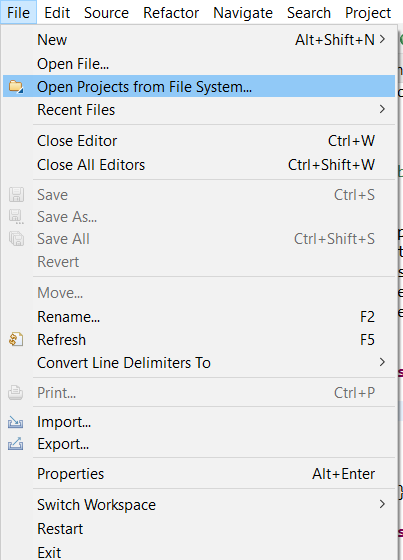
\includegraphics[scale=0.6]{Imagenes/Open Projects from File System.png}
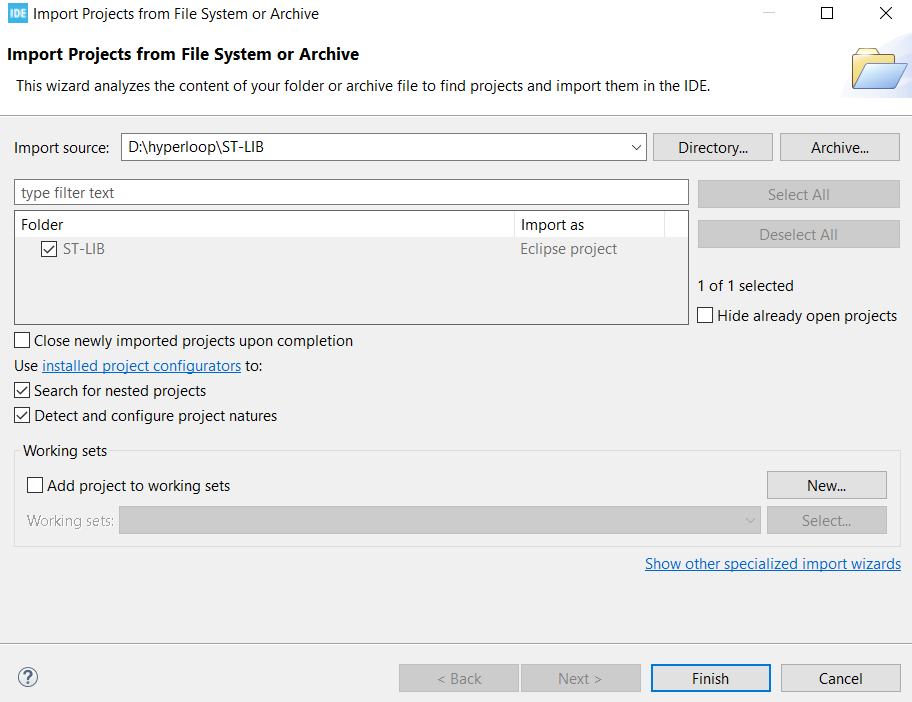
\includegraphics[scale=0.5]{Imagenes/importing ST-LIB.png}
\caption{Imagenes de como importar la ST-LIB en el cube}
\label{STLIBimport}
\end{figure}

tendrás la opción de crear un proyecto nuevo desde cero, que te dejara seleccionar tu microcontrolador y te construirá un .ioc con la configuración estándar para este, el cual tendrás que modificar a tu gusto. Aunque crear el proyecto desde cero y luego importar la librería sea posible llevara bastante tiempo debido a que habrá que configurar los periféricos en el .ioc y crear un archivo runes de configuración de la librería, así que para el caso de los microcontroladores H7 existe ya un proyecto configurado que se puede importar usando git y la opción de abrir un proyecto desde un sistema de archivos. \par \vspace{0.3 cm}

Este proyecto se denomina template-project, y como se menciona en el apartado anterior, se puede descargar en su respectivo github \cite{web:github:templateproject}. Lo que contiene este proyecto es un .ioc configurado para funcionar con la ST-LIB, junto a módulos de la HAL modificados y un archivo runes que tiene múltiples periféricos de ejemplo listos para utilizar. \par
El mayor defecto de la librería es que requiere de modificar los métodos de inicialización de los archivos generados automáticamente por el cube para que añada todos los periféricos como los desea el usuario lo cual aumenta mucho la complejidad de uso y puede lastrar el proceso de creación de código. Por ello se ha creado el template project con el propósito de ofrecer una versión utilizable directamente nada más se descarga, pero esta viene con sus propios problemas. Principalmente, la configuración de pines con la que viene es estática, así que si se usa otra familia o se quiere cambiar la función de un pin por cualquier razón, se debe modificar todos estos archivos obligatoriamente. \par
Se ha intentado ofrecer todas las utilidades posibles en la configuración del template-project, pero más adelante se vera un apartado de como modificarlo para cambiar configuraciones comunes. \par \vspace{0.3 cm}

Ahora se deberá importar el template-project en el cube. Lo primero que se debe hacer si se le cambia el nombre al template-project es modificar el .project que se encuentra dentro de la carpeta del proyecto. Dentro de este archivo hay una línea que pone <name>, y ahi se deberá poner el nuevo nombre del proyecto exactamente igual. Si no se cambia, el cube simplemente no lo importará cuando se apriete al botón de importar. \par \vspace{0.3 cm}

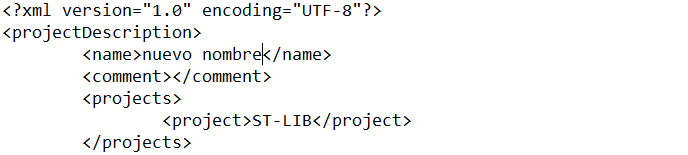
\includegraphics{Imagenes/cambios project.PNG}

\par \vspace{0.3 cm}
Además de el .project, la carpeta en la que se encuentra y el .ioc deben tener este nombre, y no se puede tener importado en el cube otro proyecto que se llame igual (o que tenga su .ioc o su <name> dentro del project igual). En cualquiera de estas situaciones, el cube no importará nada y no lanzará ningún error. Una vez todo se haya modificado para que coincida, se selecciona de nuevo la opción de \textit{``Open projects from file system''} y se importa de la misma forma que la ST-LIB. Si al importarlo no aparece en el workspace inmediatamente lo más probable es que haya un error de los mencionados previamente.  
\par \vspace{0.3cm}
Una vez tanto la ST-LIB como el proyecto estan importados correctamente al workspace del cube queda tocar una última configuración antes de comenzar a programar. La ST-LIB está pensada para funcionar tanto en las nucleos comerciales como en placas diseñadas con un cristal de cuarzo externo. Esta configuración se ha de introducir al programa en tiempo de compilación, y como el cube usa su compilador interno para hacer esta tarea debe indicarsele en el propio proyecto las variables ambiente que se usan. 
\par \vspace{0.3cm}
Poniendo el cursor encima del proyecto ST-LIB importado, se pulsa el botón derecho del ratón, se selecciona \textit{``properties''}, y dentro de C/C++ general > Path and Symbols > Symbols se modifican tanto GNU C como GNU C++. En el primero se pone en HSE la frecuencia del timer global del microcontrolador deseado (para las nucleos de la familia H7 es 8000000MHz, y se escribe como 8000000UL) y se dejan los símbolos tanto de NUCLEO como de BOARD sin ningun valor asociado. En GNU C++ se deja solo el símbolo que represente la configuración deseada, NUCLEO para usar el cristal de cuarzo interno y BOARD para usar un cristal externo (timers HSI y HSE respectivamente). \par

\begin{figure}[h]
  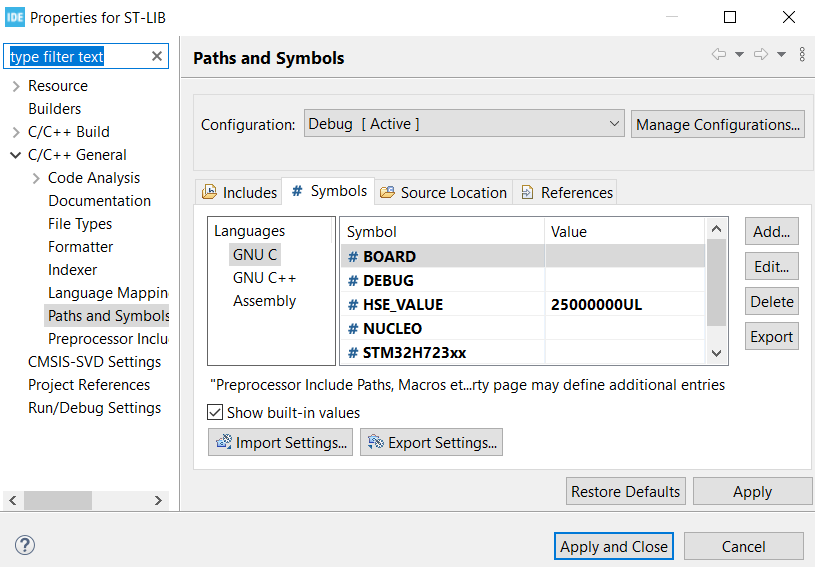
\includegraphics[scale=0.45]{Imagenes/Modificar Simbolos ST-LIB.png}
  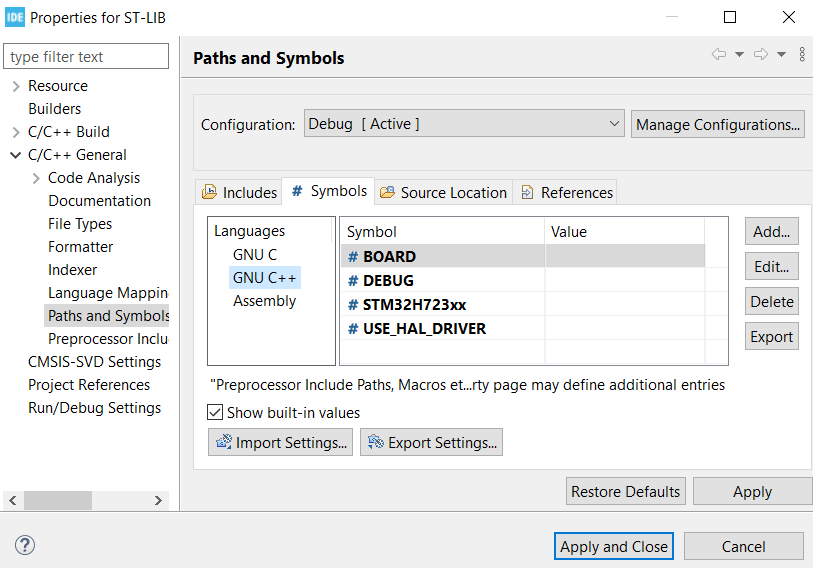
\includegraphics[scale=0.45]{Imagenes/Modificar Simbolos ST-LIB++.png}
  \caption{Ejemplo de configuración para una placa con cristal externo a máxima velocidad de un microcontrolador H7}
  \label{configSTLIBenviroment}
\end{figure}

Luego se aplican las mismas modificaciones en el proyecto y ya estaría listo. Solo quedaría probar si los timers estan configurados correctamente, la forma más facil de hacer esto es hacer que un LED conocido parpadee cada segundo usando el módulo timer y comprobar que efectivamente no parpadea ni demasiado lento ni demasiado rápido. 


\newpage

\section{Desarrollo de la librería}

En esta sección se vera una memoria de como se desarrollo la librería, explicando las condiciones sobre las que se trabajaba, los objetivos principales de la librería \par


\subsection{Métodos de gestión de proyecto}
Para estructurar un proyecto en grupo se necesita una organización clara. La jerarquía del equipo usada fue una estructura organizativa funcional de poca verticalidad. Se requiere de una estructura organizativa funcional debido a que el proyecto Hyperloop es multitudinario, y los sub-sistemas deben saber a quien dirigirse a partir de su competencia cuando requieren a personas de campos específicos. El proyecto de la ST-LIB entraba dentro de el sub-sistema de firmware, y requería de comunicación directa y continua con el equipo de software y hardware para conocer las especificaciones funcionales necesarias que debía cubrir la librería. \par\vspace{0.3 cm}
Esta estructura se dividió en tres capas, los miembros y colaboradores del equipo, los PM \textit{(project manager)} que gestionaban un sub-sistema entero, y los capitanes que dirigían a todo el equipo a partir de comunicarse principalmente con los PM y para casos específicos directamente con los miembros y colaboradores más instruidos en la tarea. Aunque hubiese una jerarquía de equipo se dejaba abierta la comunicación directa entre todo miembro del equipo, y se usaba la responsabilidad y confianza en los miembros como único muro para no abrumar a los PM y capitanes con dudas y consultas varias. Este tipo de método de trabajo, si se consigue llevar a cabo, es muy ágil y flexible, pero es más vulnerable a fallos individuales y puede llegar a sobrecargar a miembros del equipo clave si no se trata con cautela. Se requiere de personas capaces de trabajar en equipo, así que la instrucción para este tipo de metodologías es obligatoria para cada nuevo miembro. 
\par \vspace{0.3 cm}
Para el sub-sistema de firmware se uso específicamente una metodología scrum ágil basada en fases de proyecto con sprints e hiatos de planificación para las consecuentes fases y para tratar posibles retrasos. En cada sprint se le asignaba a cada miembro unos trabajos que se debían llevar a cabo en un marco de tiempo, y al final de este se revisaba cuantos de estos objetivos se habían cumplido y se trataban los posibles retrasos así como se aprovechaban los posibles adelantos redistribuyendo trabajo. \par \vspace{0.3 cm}
Esta metodología pone responsabilidad en cada miembro al tener una forma objetiva de marcar su trabajo. Lo bueno de esto es que permite aligerar la carga de trabajo de los PM y capitanes que debido a la estructura de equipo corren riesgo de sobrecarga. Lo malo es que al ofrecer una parte del trabajo a cada miembro y planificar teniendo en cuenta lo que van a completar un miembro disfuncional, ausente, o que sufra un contratiempo puede provocar un fuerte cuello de botella y dañar el ritmo del equipo entero. \par
Para mitigar lo máximo posible la rotura del ritmo de trabajo, los sprints se reducen a una semana de tamaño, haciendo reuniones a mediados y final de sprint para redistribuir el trabajo y analizar los avances, permitiendo rectificar problemas en el avance del trabajo en pocos días, siempre y cuando los miembros sean comunicativos.
\par \vspace{0.3 cm}
En cuanto a las fases del proyecto, que definen hitos importantes del avance del proyecto, se dividen en fase de diseño, fase de testing y fase de presentación. La fase de diseño incluye la construcción del equipo, la comunicación de requisitos, el diseño de la estructura de la librería y la implementación mínima funcional de esta, en ese orden. Como esta fase de diseño sucede a la vez que la fase de diseño de otros sub-sistemas, es común la retroalimentación de requisitos y la reestructuración de la librería mientras se esta en fases más avanzadas, por problemas que se puedan encontrar o mejoras posibles que se puedan añadir. Ahí es donde brilla la naturaleza iterativa del scrum, permitiendo añadir a los sprints cambios de la estructura y comunicarlos rápidamente al equipo sin afectar al ritmo de trabajo. \par \vspace{0.3 cm}
Una vez se termina la fase de diseño se hace un release de la librería (mas adelante se elaborara en el concepto de release) con una funcionalidad probada mínima y puede comenzar la fase de testing. Esta fase es la más intensa debido a que es aquí donde se encuentran la mayoría de errores y contratiempos. Se basa en utilizar la librería para implementar múltiples placas con requisitos funcionales críticos usando todas las herramientas de la librería y hacer pasar a estas placas unos tests tanto de seguridad como de capacidades funcionales. \par
Es posible que en esta fase se requieran cambios en el diseño de la estructura de la librería como el añadido de nuevos módulos o mejorar las capacidades de módulos ya existentes, lo cual puede afectar a su vez a otros módulos de la librería provocando un efecto cascada de trabajos urgentes y fallos en la librería. Por ello en esta fase se requiere de horarios flexibles, una comunicación muy abierta, y de trabajo preventivo. En esta fase se hacen múltiples releases que arreglan errores, añaden funcionalidades y confirman revisiones al código. Al terminar esta fase la librería debe estar en su versión final, debe cumplir todos los requisitos y estar lista para actuar en sistemas críticos. \par \vspace{0.3 cm}
La ultima fase es la fase de presentación, que dura alrededor de un mes. Aquí se junta el trabajo de todos los sub-sistemas, se termina el producto, se planifica las formas de actuar a la hora de la presentación y finalmente se presenta en la EHW. Esta fase seria la equivalente a los meses después de la salida al mercado de un producto, donde el equipo recibe feedback y hace unos cambios mínimos de ultima hora para arreglar fallos que no se pudieron ver sin tener el producto final. Si por alguna razón se requiriesen cambios drásticos en la librería, querría decir que la metodología de trabajo ha fallado. 

\subsection{Gitflow}
El Gitflow es una rama de la metodología de gestión de proyectos orientada principalmente a el control de archivos y documentos del proyecto, pero como esta parte es tan esencial en un proyecto de desarrollo de software como lo es la creación de una librería, se le ha dado un apartado propio para evitar saturar la sección de métodos de gestión de proyectos. 
\par \vspace{0.3 cm}
Gitflow es una estructura y planificación de el uso de programas de gestión de versiones (principalmente Git, del cual viene su nombre) que define los pasos a seguir para añadir cambios o introducir nuevos archivos al espacio de trabajo del equipo sin interferir en el trabajo de otros.
El Gitflow se basa en el uso de ramas \textit{(o ``branches'')} de trabajo que se encargan de controlar partes especificas de los documentos (en nuestro caso, los módulos de la librería) que hacen una instantánea de el estado actual del espacio de trabajo y te deja modificar esta instantánea sin afectar al espacio en común del equipo, y por ende evitando daño directo al avance de los compañeros. Una vez se ha terminado de trabajar en la rama, se debe reunir los avances hechos con el espacio de trabajo del equipo, en un acto conocido como fusión de las ramas \textit{(o ``merge'')}\par \vspace{0.3 cm}

En nuestro espacio de trabajo en común esta compuesto por dos ramas, \textbf{development} que guarda todos los avances que fueron mergeados, y \textbf{main} que guarda la ultima instantánea del proyecto que ha sido correctamente testeada y su funcionalidad esta asegurada. \par
Para poder juntar los avances hechos por un miembro del equipo con development \textit{(la rama de trabajo en común)} se debe tener un mínimo de control para asegurar que no se ha cometido un fallo que comprometa la funcionalidad de la rama development. Para ello se usa las \textbf{pull-request}, una funcionalidad de Git que permite a otros miembros del equipo que no hayan trabajado en esa rama revisar los cambios, pedir modificaciones a la rama a fusionar, y finalmente aceptar los cambios. En nuestro caso en concreto, se requería que la mitad del equipo de firmware (2 personas + el propietario de la rama) aceptara la pull-request de la rama. \par
Para hacer una nueva release \textit{(fusionar development con main)} se reúne al equipo entero en una reunión especial y se hace una pull-request que requiere de la aceptación del 70\% del equipo (todos menos 1) para completar esta. 
\par \vspace{0.3 cm}

Una vez la librería esta completa comienza la fase de testeo, donde el Gitflow se modifica para facilitar lo máximo posible la salida y aprovechar las nuevas herramientas que se fueron desarrollando en paralelo a la librería. Para ello lo primero que se hace es reducir el numero de personas que aceptan la pull-request para mergear a main en 1 más la herramienta de testeo automático (un servidor desarrollado para la fase de testing que corre pruebas en el código del pull request para comprobar que el código no se rompió en los cambios de esta, funcionando 24 horas). Esto reduce mucho la dependencia entre los programadores de la librería permitiéndoles sacar mucho más rápido los fixes. \par
Además se implemento un control de versiones de la rama main, permitiendo tener varias versiones funcionando al mismo tiempo; principalmente para el caso en el que una placa funcionase completamente con una versión pudiera congelarse sin tener que revisarse para las nuevas versiones, aunque también como seguro en caso de que un merge estropeara la librería de una forma imprevista ya que el control sobre la rama main fue reducido a favor de mayor facilidad a la hora de revisarla. \par
El último cambio al Gitflow entre las fases de desarrollo y testeo fue añadir como requisito a las actualizaciones a main un log file que explicara los cambios que se han producido en la librería a nivel funcional con cada nueva actualización. Estos cambios además no debían afectar a la interfaz de la librería a menos que fuese absolutamente necesario. 
\par \vspace{0.3 cm}

En cuanto a los programas usados para aplicar el Gitflow los principales fueron Git, GitHub, Visual Studio Code, GitKraken, y el formato MarkDown para la escritura de la Wiki del proyecto. En Git se usaban dos repositorios separados, uno para la propia librería y otro para el proyecto de las placas que servía, entre otras cosas, para probar la librería. Había una dependencia unidireccional entre la librería y el proyecto de los microcontroladores, por lo que el segundo debía actualizarse rápidamente a los cambios del primero. Para modificar este ultimo, se usaba un Gitflow más simplificado sin pull-requests, permitiendo cambiar mucho más rápido el proyecto de las placas a cambio de tener el riesgo de que este fallara. Este riesgo era únicamente aceptable gracias a que la librería no dependía del susodicho, y por tanto los fallos en el proyecto de las placas no afectarían gravemente al avance del trabajo. \par
Respecto a GitHub, Visual Studio Code y GitKraken eran soportes de alto nivel para facilitar el uso y entendimiento de Git a los miembros del equipo menos versados en el uso de esta herramienta. Visual Studio Code permite hacer cambios rápidos y controlar conflictos de forma más visual en las ramas, y tiene atajos para las acciones más usadas dentro de Git. GitKraken permite observar de una forma más \textit{``user friendly''} los movimientos entre ramas para ver si estaban habiendo problemas a la hora de aplicar el concepto del Gitflow en la practica. Se podían ver de que ramas a cuales se habían hecho los merge y los pull-request, permitiendo alertar branching excesivo y resaltando las ramas más problemáticas. GitHub cerraba el circulo ofreciendo control sobre las pull-request, los comentarios, y dando la capacidad de modificar la estructura del Gitflow en minutos en caso de necesidad.
\par \vspace{0.3 cm}
Los módulos de la librería (que en el Gitflow son tratados como ramas) se separaron en tres grandes bloques según su nivel de abstracción: Core, Low y High. Cada nivel requería de distintos conocimientos y cantidad de comunicación, además de que cada nivel superior tenia dependencias con los niveles previos. Para que esto fuese posible, se requiere que el grafo de dependencias entre módulos de la librería cumpla unas normas, debe ser un grafo multinivel, cuyos niveles sean los tres bloques. Esto quiere decir, a grosso modo, que ningún módulo de la librería puede depender de otro módulo del mismo nivel o de un nivel superior. Diseñar la librería así tiene otra gran ventaja añadida, y es que mientras se siga este concepto de diseño es imposible sufrir dependencias cíclicas, pues para que un grafo sea multinivel debe, entre otras cosas, ser acíclico. \par
La ST-LIB Core es el bloque que requería más conocimientos de hardware y firmware para ser creada, abstraía directamente los registros de Hardware, apoyándose únicamente en la HAL, la cual requiere de conocimientos tan amplios como trabajar directamente con los registros. Esta es la que tendría más peso en la eficiencia del código, la seguridad, y la flexibilidad de este. La mayor ventaja es que es un punto de apoyo para las capas superiores y no esta diseñada con la intención de ser usada directamente, así que podía ser tan obtusa y fea en su uso como fuese necesario para cumplir los requisitos dados por los otros sub-sistemas. \par
La ST-LIB Low es la capa intermedia entre el usuario y el corazón de la librería, y su objetivo principal es traducir a conceptos de lenguajes más abstractos las herramientas dadas por la ST-LIB Core. Pasar de uso de ids y registros a estructuras, clases y POO, gestionar los posibles fallos y recuperarse de errores o datos aberrantes, ayudar a debuggear el código al usuario, y hacer macros de estimaciones y cálculos usados en múltiples capas son algunas de las funciones que tiene esta capa. \par
Por ultimo, la ST-LIB High tiene como objetivo juntar todos los módulos de la ST-LIB Low en grandes macros como \textit{``iniciar''}, \textit{``terminar''}, \textit{``bucle de trabajo''}, o \textit{``interrupción''}, así como activar o desactivar los módulos que están en uso, y imponer protecciones entre módulos, y facilitar la creación de macros especificas para cada placa. 
\newpage

\section{Diseño y funcionalidad}
En esta sección se explicara en más detalle la estructura de la librería, como funciona y cuales son los casos de uso esperados para cada uno de sus módulos. Se dividirá en las tres partes principales de la librería: Core, Low y High, más una explicación generalizada del objetivo de diseño. 
\subsection{ST-LIB Core}
\subsubsection{Modelos y Servicios}
La ST-LIB Core se divide en la parte estructural (o los modelos) y la parte funcional (o los servicios). Los modelos permiten abstraer el concepto de registros de periféricos, relojes, contadores, uso de la memoria flash, y demás propiedades del propio hardware del micro que pueden ser demasiado abrumadoras para una persona que se esta introduciendo al mundo del firmware y demasiado repetitivas y laboriosas para un equipo que ya conoce sus necesidades sobre estos aspectos del hardware y prefieren tener una base ya creada para no tener que configurar cada proyecto que hagan. \par \vspace{0.3 cm}

Los servicios por su parte abstraen las macros más comunes en el mundo del firmware, como iniciar periférico, crear interrupción, atender interrupción, reconfigurar reloj, crear alarma, atender alarma, y lecturas y escrituras de todo tipo. Los servicios de la ST-LIB Core son primitivos y de un nivel de abstracción muy bajo, y solo existen como soporte para niveles de abstracción superiores y como opción a configurar para expertos de firmware. Las funciones que hacen son muy simples, pero reducen la necesidad de 9 lineas de código a 1, y gestionan los errores más comunes cuando se hacen proyectos a gran escala con múltiples micros como lo son no haber declarado o iniciado un Pin, equivocarse en un numero y llegar a valores peligrosos para el micro, o usar un Pin configurado de una forma para una función que requiere otra configuración. \par \vspace{0.3 cm}

La mayoría de veces gestiona estos errores a través del ErrorHandler, una clase que se dedica específicamente a dar información retro-alimentada al programador a partir de mensajes en el protocolo de comunicación preferido (Viene configurado para usar el protocolo FD-CAN, pero con un cambio a dos lineas de un método se pueden usar cualquier otro de los protocolos ofrecidos por la librería), y de parar el micro en caso de fallo de una forma más segura en lugar de usar un \textit{Hard Fault}. 

\subsubsection{Pin}
La clase Pin es el primer nivel de abstracción sobre la librería HAL y el código C con registros. Es una estructura de datos cuyo propósito es que los usuarios puedan identificar el Pin rápidamente en el datasheet y escribirlo directamente en el código sin tener que hacer traducciones ni convocar métodos. Esta pertenece a los Modelos de la ST-LIB Core.
\par \vspace{0.3 cm}
Esta estructura se encarga de abstraer el concepto de los pines de la micro en su totalidad. Lo primero que hace es mapear los valores de registro de los pines a unos valores más entendibles para el humano, usando los nombres que se le dan en la núcleo para ello. Por ejemplo, si a la configuración del pin A5 se accede con el registro \textit{0x400000001802000000000020} permite al usuario obtener este registro dando los valores A y 5 a los enum\footnote{Un enum es una estructura de C que se dedica a enumerar distintos valores para distintos nombres, similar al concepto de una variable o un mapa pero se soluciona en tiempo de compilación, por lo que no afecta a la velocidad del programa}   GPIOPin y GPIOPort. 
\par \vspace{0.3 cm}
También mapea de la misma forma las posibles configuraciones que puede tener un Pin. Para eso utiliza hasta tres enum mas; uno para saber si esta ya configurado, otro para saber que configuración tiene, y uno tercero para indicar configuraciones especiales en caso de que los modos más comunes no sean lo que se busca. 
\par \vspace{0.3 cm}
Su ultima funcionalidad es la capacidad para registrar e iniciar cada uno de los pines a partir de los métodos inscribe() y start(). Estos métodos también añaden una capa de abstracción adicional ya que inscribe acepta directamente el nombre del pin y lo traduce a los valores necesarios para obtener su dirección de registro. Con este método se puede usar directamente inscribe(A5,ANALOG) en lugar de tener que obtener la dirección de memoria de la configuración usando A+5 y usar un writemem para introducir la configuración a mano. El método start() usa los valores introducidos en el inscribe para cada Pin para completar la configuración añadiendo todos los extras necesarios, como lo son DMA, relojes y la asignación de espacio de memoria para guardar las variables. Si start() se quedara sin relojes o canales DMA para asignar a los pines configurados usaría el ErrorHandler para avisar al programador, pero esta probabilidad es ínfima pues requeriría configuraciones muy especificas (\textit{como ya explicaremos en la clase Time}). \par \vspace{0.3 cm}
Como añadido adicional, existen construidos ya todos los pines que hay disponibles en los micros de la familia H7 como estructuras de datos publicas, con los alias de P+\textit{puerto}+\textit{pin}. Por ejemplo, el pin A5 es accesible a través de un extern\footnote{extern es una palabra clave de C++ que permite indicarle al compilador que te refieres a una instancia de la variable que ya existe en otro documento, en lugar de querer crear una instancia nueva con el mismo nombre en el documento actual} como \textit{PA5} 

\subsubsection{DMA}
El concepto de Direct Memory Access (DMA) viene de la necesidad en sistemas críticos de aliviar la carga del procesador. Como un porcentaje considerable del tiempo de ejecución es consumido gestionando los accesos a memoria y los datos recibidos a través de los periféricos, se decidió que seria más efectivo crear una unidad especial de asistencia al procesador en estas acciones antes que gastar recursos en aumentar más la potencia de este. \par \vspace{0.3 cm}
DMA es entonces la abstracción del uso de un hardware especializado que puede conectarse directamente a la memoria para transferir datos por un bus. En un principio solo hacia un acto muy primitivo, mover datos de un lugar a otro, en un rango de memoria limitado con la opción de ciclar dentro de este rango de memoria o terminar su ejecución y requerir reconfigurarse cuando llenase el buffer. Sin embargo, viendo lo efectivo y barato que era implementar los DMA, con los años se fue añadiendo más canales de direct memory access a los microcontroladores y se les dio mayor capacidad de calculo, permitiendo incluso aplicar cálculos simples o relegar funciones a otras unidades de hardware y esperar su respuesta para guardarla dentro de lugares de memoria más específicos. 
\par \vspace{0.3 cm}
Mientras que el uso de DMA no es necesario para hacer nada, aprovechar esta tecnología puede mejorar mucho la eficiencia de los procesos del micro al poder ceder decenas de lineas de código que gestionan información de forma iterativa de la unidad de proceso a las unidades de DMA especializadas. Por ello, se necesitaba una abstracción de los canales DMA en la librería para poder aumentar su eficiencia en todos los periféricos que pudiesen hacer uso de esta. \par \vspace{0.3 cm}
El modelo de la DMA de la librería es bastante simplista, y deja mucha libertad y cosas por configurar a las clases de mayores niveles de abstracción ya que esta utilidad es aplicable a una plétora de casos y no es estrictamente necesaria para ninguno de estos. Se dedica a definir con enum los canales de DMA, usar un mapa para guardarse los canales libres y los canales usados, y ofrecer un método de inscripción de DMA que asigna el primer canal libre o permite, en su lugar, elegir al programador uno especifico. Luego tiene el método start() del que prácticamente todas las clases de la ST-LIB Core gozan y simplifica el inicio de estos servicios. 

\subsubsection{Paquetes}
La estructura de paquetes puede ser probablemente la clase de la librería más difícil de comprender a primera vista. Debido a la complejidad de abstracción del concepto de paquete conservando su polimorfismo, el modelo packets (paquetes en ingles) usa templates\footnote{los templates son una palabra clave de C++ para funciones, variables y clases por igual que permite decirle al compilador que el objeto al que se le asigna funciona para más de un tipo de variable. Los templates pueden indicar que funciona para todas las variables numéricas, para todas las variables que guarden un valor, o para variables dentro de una clase definida por el usuario, permitiendo una gran expresividad y polimorfismo sin requerir centenas de lineas de código} infinitos recursivos para auto estructurarse en compilación dependiendo de las necesidades vistas en el código. 
\par \vspace{0.3 cm}
Como esta clase es tan compleja, esta diseñada inicialmente como una \textit{``caja negra''}, es decir, no hace falta entender como funciona para poder usarla. Simplemente al declararse un paquete debe indicársele que tipos de variable guarda y cuantas, y luego usarse un método para o bien recibir un paquete desde un periférico y guardarlo dentro de la variable paquete creada; o bien meter valores dentro de la variable paquete (que también se puede hacer durante la construcción mediante su constructor), y enviar el paquete a través de uno de los periféricos con los servicios de comunicación que más adelante se verán. 
\par \vspace{0.3 cm}
Sin embargo, aunque no haga falta comprender el modelo Packets para poder usarlo, en el resto de esta sección se tratara de explicar como funciona. Si no se tiene comprender su funcionamiento o si se tiene una idea suficiente de su estructura con la explicación de arriba, puede pasar a la siguiente sección. En el caso de que quiera entender como funciona la explicación comienza en el siguiente parágrafo. 
\par \vspace{0.3 cm}
Como se ha mencionado arriba, el modelo de paquetes debe ser capaz de almacenar cualquier tipo o tipos de variable, en cualquier tipo de combinación, y guardarlos como un objeto paquete. A nivel de programación, esto quiere decir que debe ser capaz de recibir como parámetro cualquier combinación de tipos de variable, traducirlos a un valor binario para poder enviarlas a través de cualquier protocolo de información, y luego poder traducir de vuelta ese valor binario a los tipos de variable indicados para cerrar el concepto de comunicación por paquetes. Se requiere entonces que sea un modelo template para poder recibir cualquier tipo de variable que se pueda traducir a binario \textit{(como a nivel de hardware todo esta traducido a binario, se sabe que cualquier variable tiene al menos una forma de traducirla a binario)}, y se requiere que pueda hacer pattern matching infinito pues de antemano se desconoce cuantos parámetros van a darle al paquete. \par \vspace{0.3 cm}
Todos los métodos están sobrecargados para dos tipos de parámetros, o bien cualquier cantidad de parámetros mayor o igual que 1, o bien ningún parámetro. Este diseño esta hecho a propósito para poder definir las funciones de los métodos como series geométricas, con su caso base (0 parámetros) y luego el caso de n parámetros. Al igual que las series geométricas, una función se define por una cantidad de operaciones más la misma función pero de n-1 valor (o parámetros, en este caso). Así, un paquete de 4 parámetros se define por la traducción del primer parámetro más la definición de un paquete que contenga los otros tres parámetros. Se traduce el primer parámetro, y se convoca un paquete con tres parámetros que traduce el primero de sus parámetros y convoca a un paquete con dos parámetros. Así hasta llegar a 0 parámetros, donde se retorna el valor base (que es nada, pues el paquete esta vacío) y cuando termina su convocación el paquete de un parámetro concatena su traducción a la del paquete de 0 parámetros, y termina también la convocación del paquete de un parámetro, llegando a hacer una cadena recursiva desde los parámetros requeridos hasta 0 y de vuelta a los parámetros requeridos. Básicamente estos templates permiten hacer declaraciones recursivas en tiempo de compilación (luego en tiempo de ejecución también deberán hacerse convocaciones recursivas debido a que la palabra clave inline no funciona con los templates, pero solo sera necesario en la construcción del paquete y en las traducciones)
\par \vspace{0.3 cm}
Ahora pasaremos a explicar como maneja los cast de las variables a binario. Aunque todas las variables tengan al menos una forma de transformarse a binario, esto no quiere decir que esta forma este codificada para el uso del programa o que sea la forma de cast más sencilla y eficiente. Por ello, la clase PacketValue sirve de soporte para la clase Packet y maneja los posibles valores que puede recibir como parámetros dependiendo de algunas propiedades que puedan requerir. Esta es una estructura de tipos que define grupos de tipos y dependiendo de a que tipo pertenezcan usa un método de traducción u otro. Los separadores de grupos definidos son isContainer y isIntegral, generando los grupos Container, Integral y CustomButNotContainer. Los que pertenecen al tipo isIntegral tienen una traducción directa a binario dada por C que esta demostrada ser la más efectiva. Los que pertenecen a isContainer quiere decir que en verdad guarda más de una única variable, como una array, un mapa o un paquete (ofreciendo la opción de anidar paquetes dentro de paquetes). 
\par \vspace{0.3 cm}

\subsubsection{Periféricos básicos: Analog y Digital}
Analog y Digital en concepto son sencillos, y la mayoría del tiempo se pierde en configurarlos. Por ello, en la librería Core hemos creado las clases Analog, DigitalInput, DigitalOutput y EXTI principalmente para facilitar esto. \par
La estructura de los tres primeros es la misma: mapas que alocan los recursos de la placa y los metodos inscribe, start, y get value/set state que permiten configurar un pin (ya definido en la clase Pin) y recibir la id de la configuración, inicializar todos los pines, y hacer una orden de lectura/escritura en los periférico. En este nivel aun se deben gestionar id's pero en la ST-LIB Low se pone una capa más de abstracción para tenerlo como un objeto de una clase. 
\par \vspace{0.3 cm}
Para utilizarlo es tan sencillo como parece, primero convocas inscribe dandole como parametro el Pin que deseas configurar, y guardando su retorno en una variable uint8, luego convocas el start y por último tomas las lecturas cada vez que las necesites. Aquí un ejemplo del main:

\begin{lstlisting}
uint8_t DigitalID = DigitalInputService::inscribe(PA5);
uint8_t AnalogID = ADC::inscribe(PA0).value(); #devuelve un optional
uint8_t OutputID = DigitalOutputService::inscribe(PC0);
HALAL::start(); #macro que contiene todos los metodos start necesarios
while(1){
  DigitalOutputService::set_pin_state(1);
  printf(ADC::get_value(AnalogID));
  printf(DigitalInputService::get_value(DigitalID));
}
\end{lstlisting}
\par \vspace{0.3 cm}
Se recomienda utilizar el HALAL start en lugar de usar los starts de los módulos ya que algunos módulos dependen de que otros hayan iniciado y tienen que activarse en un orden en concreto. Por ejemplo, el módulo ADC usa las DMA para capturar los valores sin usar capacidad de procesador para mejorar la velocidad del código, pero tiene el pequeño defecto de no funcionar si las DMA no 
\par \vspace{0.3 cm}
Aparte de estos tres sensores esta el EXTI (External Interrupt) que permite activar interrupciones directamente a partir de cableado. El EXTI es más especial porque le puedes especificar que es lo que tiene que hacer cuando sea interrumpido a traves de una \textit{lambda expression}. Las lambda son basicamente funciones sin identificador, que se define por su clausula de captura de parametros, los parametros que recibe, y el código a ejecutar. 
\begin{lstlisting}
uint8_t externalID = ExternalInterrupt::inscribe(PA5,()[]{printf("Hola");},FALLING);
HALAL::start();
\end{lstlisting} 
\par \vspace{0.3 cm}
Este código define un external interrupt en el pin PA5 que imprimirá ``Hola'' cada vez que caiga la señal; es decir, que pase de 1 a 0. Puedes ponerle las opciones de RISING o FALLING, que quiere decir de 0 pasa a 1 y de 1 pasa a 0. \par\vspace{0.3 cm}
Hasta ahora nos hemos referido a la función \textit{printf} como la función que imprime un texto, pero como el periférico por el que se imprime depende de la preferencia del programador, probablemente sea necesario sobreescribirla. Actualmente en la ST-LIB lo imprime por UART, un protocolo de comunicación del cual hablaremos en las próximas secciones. Dependiendo del modo de programación (Nucleo o Board) estara en el uart1 o en el uart2 (definidos en el Runes) \par
La librería la sobreescribe en el módulo UART (sobreescribe el metodo write el cual es convocado por printf), así que para sobreescribirla debe removerse de UART primero.

\subsubsection{PWM}
El módulo PWM (\textit{Power Width Modulated}) es un periférico especial que permite generar una señal periódica cuadrada con un periodo y un ciclo de trabajo \footnote{tiempo que se pasa activo dentro del periodo, en porcentaje. También se le conoce como \textit{duty cycle}} configurables. Estas señales son especialmente útiles para controlar motores, sincronizar comunicaciónes y simular una señal análoga con cualquier voltaje deseado. 
\par \vspace{0.3cm}
El módulo PWM tiene una clase con constructor, por lo que para usarla debe guardarse el objeto cuando haya sido instancializado. Ademas del constructor, tiene los métodos turn on, turn off, set frequency, get frequency y set duty cycle. Estos metodos activan el PWM, lo desactivan, cambian la frecuencia (y con ello el periodo) con una uint dada, obtener la frecuencia que tiene guardada, y cambiar el duty cycle. \par
Los periféricos de esta clase no se inicializan en el HALAL start como protección, ya que entre otras cosas las PWM sirven como control de motor, e inicializarlo de forma discreta podría ser peligroso. En su lugar, el usuario debe activarlo y desactivarlo cuando vea necesario. 
\par \vspace{0.3cm}
Ademas de la clase PWM, el módulo tiene tres clases que heredan de ella que añaden nuevas propiedades. Estas son PhasedPWM, DualPWM y DualPhasedPWM. PhasedPWM te permite añadir una fase angular a la onda cuadrada que genera el PWM, para sincronizar la onda con otras ondas a conveniencia. La DualPWM crea dos señales PWM negadas entre si. Y la DualPhasedPWM es una DualPWM a la cual se le puede aplicar fase (ambas son afectadas por el cambio ya que una es la negada de la otra). La fase es una float que puede ir desde -100\% hasta +100\%, que a nivel de onda representa un cambio de fase de -pi hasta +pi (en radianes). Un ejemplo rápido de uso:
\begin{lstlisting}
  DualPhasedPWM pwm(PA5,PA6);
  pwm.set_duty_cycle(40.0);
  pwm.set_frequency(1);
  pwm.set_phase(30.0);
  pwm.turn_on();
\end{lstlisting}
\par \vspace{0.3 cm}
Con este código hemos puesto dos pwm negadas entre si en un duty cycle del 40\%, una frecuencia de 1 Hz, y una fase del 30\% (+pi*0.3 de fase angular). Como se puede comprobar operar las PWM se ha vuelto mucho más sencillo ya que el módulo gestiona automaticamente toda la configuración de software.  

\subsubsection{Time}
La clase time incluye la gestión de los timers, las alarms, y el rtc (\textit{real time clock}). Como hay una cantidad limitada de timers en el microcontrolador y algunos de estos son necesarios para hacer funcionar otros módulos como las PWM, en su lugar se utilizan tres timers generales para que gestionen la gran mayoría de las alarmas y una interfaz con los timers restantes en caso de querer una alarma crítica. \par
Los timers generales low y mid estan configurados para crear una interrupción cada 50 microsegundos y cada milisegundo, respectivamente. Luego de saltar la interrupción comprueba si las condiciones de las alarmas configuradas por el usuario se han cumplido, si es el caso ejecuta la lambda expression que le corresponde y en caso contrario la ignora. Un ejemplo de configuración:
\begin{lstlisting}
  uint64_t counter = 0;
  Time::register_mid_precision_alarm(100,[&](counter){counter++;});
  Time::register_low_precision_alarm(100,[&](counter){printf(counter);});
  HALAL::start();
\end{lstlisting}
\par \vspace{0.3 cm}
Este código sumara cada 100 microsegundos +1 al contador y lo imprimirá cada 100 milisegundos. Hay que indicar que el divisor del mid precision redondea hacia abajo y su paso es 50, asi que poner menos de 50 microsegundos como intervalo de la alarma hara que no funcione correctamente. De la misma forma si se pone 75 se redondeara a 50 para que encaje en el reloj.  \par
Otro problema del mid precision timer es que requiere del timer23 de la placa; y dependiendo de el código que estes implementando puedes necesitar el timer23 para declarar PWMs en algunos pines. En el caso de la familia H7 hay 4 timers de 32 bits (el 2, el 5, el 23 y el 24). El 24 se usa para el global timer, y el 2 y el 5 estan asignados para high precision timers. Si declaras los pines que usan el timer 23 para el PWM y utilizas el mid precision timer el iniciador del timer dara un error avisando de que no puede usarse el reloj para ambas cosas, pero se debe tener en cuenta a la hora de estructurar una placa. También se puede cambiar el Runes si tu núcleo específica permite otra configuración, pero eso se tratará en su respectivo apartado. Como última medida se podría modificar el módulo time para usar uno de los relojes de los high precision timers y darselo al mid precision time, pero esto dejaría a la núcleo con solo un timer de precisión crítica \par \vspace{0.3 cm} 
Además de los timers de propósito general estan los ya mencionados global timer y RTC. Estos sirven para mantener una cohesión temporal dentro del propio código; del orden de segundos y años respectivamente. Todos los timers tienen un valor máximo antes de que hagan overflow en su contador y vuelvan a 0. Esto permite por un lado tener un activador por hardware para interrupciones sin necesidad de implementar circuitería que aumente el precio (el bit de overflow). Pero por otro lado hace que se pierda toda la información sobre el tiempo que ha pasado cuando este timer sufre overflow. Si han pasado 2 segundos o 1 mes es indistinguible para el timer, ambos son un valor de 0 hasta $2^{32}$, en periodos de reloj. Esto para cálculos temporales y comunicaciónes es un gran problema, pues suelen requerir estos valores para poder funcionar. Por ello se usan estos dos timers, cuyos plazos de overflow son mucho mayores para poder trabajar con ellos. \par 
El global timer guarda en nano segundos el tiempo que ha pasado desde que se inició, y tiene una capacidad de overflow de 16.84 segundos ($(2^{32})/(2,55·10^8)$, que son el rango de su contador y su frecuencia). Lo bueno de este reloj es su gran precisión para calculos críticos y su cercanía al hardware. Lo único malo es que los propios calculos deben implementar su control de overflow (hay un ejemplo con el encoderSensor en la ST-LIB LOW, que lo usa) y que solo funciona para calculos que trabajen en un rango de tiempo que no alcance las decenas de segundos. Si se quiere usar para estampas de tiempo más altas deberá hacerse un contador por encima que controle cuantas veces se ha hecho overflow, además de que su drift de reloj puede comenzar a acumularse. \par \vspace{0.3cm}
El RTC (Reloj de tiempo real o Real Time Clock) es un reloj que guarda estampas de tiempo en el formato de fechas. Contiene contador (que se puede traducir a milisegundos), segundos, minutos, horas, dia, mes y año; y su capacidad hasta el overflow es de 99 años, ya que tiene 8 bits alocados para guardar el año en BDC \footnote{BDC o Binary Coded Decimal es un formato alternativo a la int en el que se usan cuatro bits para expresar cada cifra de un numero, haciendo que se escriba igual en decimal que en hexadecimal. Así por ejemplo, 13 se escribe 1101 0x0C en binario y 0001 (1) 0011 (3) o 0x13 en BDC. }. El RTC se puede configurar para que use un generador de señales externo, para usar el cristal de cuarzo interno del micro, o para usar cualquiera de los 24 relojes como su generador de señales de reloj. De base esta configurado en la librería para usar el cristal de cuarzo ya que tiene un desfase y un drift conocidos y documentados para todos los microcontroladores de la familia. \par 
El RTC esta pensado principalmente para hacer estampas de tiempo en comunicación entre placas o con clientes externos, y es especialmente útil ya que se puede sincronizar con otros agentes a traves del protocolo ntp directamente. El rtc se inicia automaticamente con el st-lib start y esta pensado para actualizarse usando ntp, pero tiene un método set rtc para que se actualice desde código si la conexión por ethernet no es posible.

\subsubsection{CORDIC}
El módulo CORDIC es una librería que aprovecha la unidad de calculo interna con el mismo nombre. Es una librería de aceleración de calculo trigonométrico la cual supera incluso a la librería arm math hecha para calculo por estimación en arquitecturas de microcontroladores. La razón por la que esta pequeña unidad la supera es porque esta diseñada específicamente para aplicar el algoritmo de Volder, especializado en funciones trigonométricas e hiperbólicas. \par
La mayoría de las familias de microcontroladores STM incluyen la unidad de aceleración CORDIC, pero si el micro no lo incluye esta librería no funcionara y se deberá desactivar el módulo dentro de la HAL (normalmente si tu microcontrolador no tiene CORDIC la flag de CORDIC MODULE esta ya desactivada, apareciendo el código dentro de los ifdef en grís).
\par \vspace{0.3cm}
Una de las peculiaridades del CORDIC es que solo funciona con lógica binaria; es decir, no acepta coma flotante (ni floats ni doubles). El módulo CORDIC ya viene con un metodo que transforma las float (en radianes) a int32 en el formato que el CORDIC recibe. Sin embargo, no se recomienda abusar de este método ya que la transformación de int a float consume muchos recursos desde el punto de vista de la optimización (estamos hablando a nivel de ciclos de reloj), haciendo que vaya más lento incluso que la librería math arm con lógica de floats, lo cual le quita el sentido a usar el módulo CORDIC en primer lugar \footnote{hay que añadir que la familia H7 es la más potente de todas las familias, y la unidad CORDIC interna es la misma para todas las familias y su cálculo independiente del reloj del microcontrolador. Esto quiere decir CORDIC sera más útil para otras familias y este módulo podría superar math arm incluso con recasting continuo en estas (porque un ciclo de reloj toma más tiempo y por ende CORDIC necesita menos ciclos de reloj para hacer la operación)}. \par
Por ello CORDIC solo se puede usar de forma eficiente si tienes tres o más operaciones trigonométricas consecutivas que aplicar a un valor antes de tener que volverlo a transformar o si se usa lógica binaria en todo el código conectado a los cálculos trigonométricos. El primer caso se vería así:
\begin{lstlisting}
double angle = pi * 0.5;
int32_t unary = RotationComputer::radian_f32_to_q31(angle); 
int32_t *pointer1 = &unary;
int32_t *pointer2;
int32_t *pointer3;
RotationComputer::cos_and_sin(pointer1, pointer2, pointer3, 1);
RotationComputer::phase(pointer2,pointer3,pointer1,1);
angle = RotationComputer::q31_to_radian_f32(unary);
\end{lstlisting} 
\par \vspace{0.3cm}
El método cos and sin recibe un ángulo a traves de su primer parametro y calcula el coseno y el seno, metiendo estos valores en los punteros out que recibe como parametros. La razón por la que usa punteros es porque puede funcionar también con arrays de valores. El último valor es, de hecho, el tamaño de la array que recibe. La otra forma de usarlo, y la más recomendable si tus periféricos te devuelven en int los valores a procesar (como suele ser el caso), es con la lógica de ints directamente:
\begin{lstlisting}
int32_t *values = values_array;
int32_t *x;
int32_t *y;
RotationComputer:cos_and_sin(values,x,y,values_array_length);
RotationComputer::phase(x,y,values,values_array_length);
\end{lstlisting}
\par \vspace{0.3cm}
Lo único tener en cuenta que hay que traducir el formato en el que se reciba los valores a el formato unario para que el cálculo sea correcto. El formato de los angulos recorre todos los valores posibles de las int, donde $180^o$ es el valor máximo que puede tener la int y $-180^o$ el valor mínimo (máximo negativo). \par
Esto tiene las ventajas de que aprovecha al máximo la precisión que le dan y que las sumas de angulos no sufren overflow, ya que la representación de los angulos negativos funciona igual que la de las ints. Por ejemplo, max int +1 es igual a -max int, y $179.99995^o + 0.0001^o = 180.00005^0 = -179.99995^o$. \par
El formato de las coordenadas simplemente representa un espacio acotado en -1 y 1 tanto en x como en y. Cuando superas el límite simplemente sufre overflow. \par \vspace{0.3cm}
Los metodos phase y modulus operan en dicho espacio. \textit{phase} mide el ángulo entre la recta formada por el punto dado y el punto de origen con el vector (1,0). Esto es especialmente útil para comparar dos angulos, ya que la fase entre ambos es \textit{``la fase del primero con el eje x - la fase del segundo con el eje x''}. Osea, se les hace fase a ambos vectores y se restan los resultados. \par
\textit{modulus} sirve para obtener la distancia entre el origen y el punto dado como un valor escalar. Como esta distancia puede ser mayor que uno (el punto (1,1); por ejemplo), y como este numero solo puede ser positivo, devuelve una uint32 en lugar de una int32 para poder llegar hasta el 2, cambiando su imagen de [-1,1] a [0,2]. Esto es importante porque \textbf{el modulus tiene sus propias unidades}, por lo cual no se puede utilizar sin más como unidad en el espacio. Si guardas el valor de retorno en una int en lugar de una uint y el resultado era mayor que 1 te devolvera un número negativo, lo cual es imposible pues las distancias (escalares) son positivas necesariamente. 

\subsubsection{Encoder}
El encoder o codificador rotatorio es un periférico que traduce señales de pulsos a posición angular representada con un contador de giros, y es muy usado en el mundo de los motores y la electrónica para obtener posición y cambio de posición a partir del diámetro de la rueda y su posición angular. De este sale también el encoder lineal, que traduce las mismas señales a desplazamientos lineales directamente (los contadores representan una distancia igual a la distancia de las bandas del encoder lineal). \par
Los codificadores relativos son una versión más pequeña y económica que obtienen unicamente el cambio de posición relativo y no la posición angular absoluta. Simplemente envian una señal ``+1'' o ``-1'' cada vez que una banda del encoder se cruca con el interruptor óptico, y suelen tener una precisión similar por una pequeña parte del precio. \par \vspace{0.3cm}
El módulo encoder se encarga de transformar estos codificadores relativos en un codificador completo, guardando la posición inicial y sumando en un contador todos los cambios de posición para obtener el desplazamiento total. También se encarga de la configuración inicial del encoder como el resto de módulos. La declaración funciona así:
\begin{lstlisting}
  uint8_t encoder_id = Encoder::Encoder(PE0, PG1).get_value();
  ST-LIB::start();
  Encoder::turn_on(encoder_id);
  while(1){
    uint32_t position = Encoder::get_counter(encoder_id);
    bool direction = Encoder::get_direction(encoder_id);
  }
\end{lstlisting}
\par \vspace{0.3cm}
Este código declara que el encoder esta conectado a los pines PE0 y PG1, lo enciende y lee de forma continua tanto la posición como la dirección a la que fue la última rotación. Tener en cuenta que el encoder comienca su contador en 32768 para que comience lo más lejos posible del overflow y el underflow, debido a que dependiendo de la dirección puede sufrir uno u otro. En los calculos que se hagan se ha de tener en cuenta que esta es la posición inicial del encoder. Además, si se tiene pensado usar en largas distancias se recomienda añadir lógica en caso de overflow (y undeflow). En la ST-LIB Low ya se añaden todas estas abstracciones.
\subsubsection{Flash}
La mayoría de la memoria del microcontrolador es volátil, lo cual quiere decir que su información es destruida cuando la núcleo se reinicia o deja de alimentarse. Sin embargo, la mayoría de los microcontroladores, incluyendo todos los de la familia H7, tienen una pequeña memoria flash de 1 MB donde se puede guardar información no volátil como el bootloader, el código y variables o información generada durante el cómputo. \par
El módulo de la flash tiene como propósito manejar esta memoria de la forma más directa y simple posible. Tiene tres métodos: Read, Write y Erase. Los dos primeros reciben una posición de memoria inicial, un puntero con o bien los datos a escribir o el lugar donde se guardaran los datos leídos, y el tamaño de la lectura o escritura (cuantos bytes se va a leer). Erase por su lado simplemente recibe la posición inicial y la final y borra todo de por medio. \par \vspace{0.3cm}
La flash se divide en páginas de 128 kB, y para escribir se debe acceder a una página de la flash en modo escritura, y cuando se accede de esta manera la memoria es borrada para poder escribir la nueva información. Para solventar esto simplemente se hace una lectura antes de la escritura, se anexiona la parte de la memoria que no se va a escribir al buffer de escritura, y se escribe toda la página.
\subsection{ST-LIB Communication}
La comunicación es en su mayoria parte de la ST-LIB Core, pero es tan extensa que por simplicidad es mejor darle su propio apartado. Al igual que la mayoria de la ST-LIB esta apoyada en la librería HAL, parte de la ST-LIB Communication se apoya en la librería LWIP, un middleware que gestiona las comunicaciones por Ethernet TCP/IP muy eficiente y que trabaja principalmente con interrupciones. 
\subsubsection{UART}
UART es el protocolo de comunicación más sencillo que implementa la librería. Su funcionamiento es bastante básico, tiene un canal para el reloj que marca el paso para enviar y leer cada bit, y otro canal para enviar byte a byte la información. 
\par
El canal se encuentra en estado lógico 1 cuando esta parado, y la comunicación se hace por paquetes de tamaño dependiente del estándar usado. En el caso del estandar 8N1 (\textit{el más usado y la configuración inicial en la ST-LIB}) se inicia la comunicación con un bit en estado 0, se envia el byte de información (el tamaño del paquete en este estándar, 8 bits), y se cierra con un bit lógico 1. 
\par \vspace{0.3cm}
En la librería UART tiene las opciones de comunicación de polling y por DMA con interrupciones, como la mayoría de módulos de la ST-LIB Core tienen. Las opciones son tan sencillas como leer y escribir, pues UART es un protocolo de comunicación punto a punto. El código por polling: 
\begin{lstlisting}
  uint8_t uart = UART::inscribe(UART::uart2);
  ST-LIB::start();
  uint8_t data_send[]{5,5,2,2};
  uint8_t data_receive[4];
  while(1){
    if(UART::transmit_polling(uart, data_send)){
      UART::receive_polling(uart, data_receive);
    }
  }
\end{lstlisting}
\par \vspace{0.3cm}
Este fragmento de código enviará continuamente los bytes 5, 5, 2, 2 y esperara a la respuesta desde el otro lado, la cual guardara en la array data receive y volvera a comenzar. Sobre el método inscribe, este recibe un periférico UART declarado en el módulo \footnote{El módulo UART solo tiene declarados diez périfericos uart (de uart1 a uart10). Si se quieren añadir más, se deberá modificar el header del módulo para declararlos} y definido en el archivo runes (en el ejemplo uart2). Como es común en la ST-LIB Core; el inscribe te devuelve un número id que representa en que punto de su lista fue guardada la configuración de tu periférico. 
\par
Importante añadir que el inscribe solo funcionará sí se hace antes del ST-LIB start. Esto es debido a que el start activa todos los periféricos inicializados por el usuario; pero una vez el ST-LIB start se ha ejecutado ya no activará más periféricos. Se puede circundar este problema con el método start de cada módulo, pero la mejor práctica es tener los periféricos fijos antes de activar el código de la placa. 
\par \vspace{0.3cm}
La versión usando DMA tiene un par de añadidos nuevos, pero también añade complejidad al código. Hay dos métodos adicionales, \textit{is busy} y \textit{has next packet}, que permiten saber si la comunicación por DMA ha terminado. El mismo código por DMA sería: 
\begin{lstlisting}
  uint8_t uart = UART::inscribe(UART::uart2);
  ST-LIB::start();
  uint8_t data_send[]{5,5,2,2};
  uint8_t data_receive[4];
  while(1){
    if(!UART::is_busy(uart)){
      UART::transmit(uart, data_send);
    }
    if(UART::has_next_packet(uart)){
      UART::receive(uart, data_receive);
    }
  }
\end{lstlisting}
\par \vspace{0.3cm}

En este caso el código hara una petición a la DMA para que trasmita los datos del data send siempre que está este libre, mientras que al mismo tiempo revisará si ha recibido un paquete del otro lado y de ser el caso lo guardara en data receive. \par En este caso no tiene mucho sentido usar la DMA porque no hay mas código que ejecutar que comunicarse por UART, pero la ventaja viene en que mientras esta gestionando el canal de comunicaciones por DMA el micro puede seguir corriendo código. \par \vspace{0.3cm}
Un ejemplo muy básico de cuando podría servir la DMA con UART es si se tiene más de un canal UART. El código sería asi: 
\begin{lstlisting}
  uint8_t first_uart = UART::inscribe(UART::uart1);
  uint8_t second_uart = UART::inscribe(UART::uart2);
  ST-LIB::start();
  uint8_t data_send[]{5,5,2,2};
  uint8_t data_receive[4];
  uint8_t data_receive2[4];
  while(1){
    if(!UART::is_busy(first_uart)){
      UART::transmit(first_uart, data_send);
    }
    if(!UART::is_busy(second_uart)){
      UART::transmit(second_uart, data_send);
    }
    if(UART::has_next_packet(first_uart)){
      UART::receive(first_uart, data_receive);
    }
    if(UART::has_next_packet(second_uart)){
      UART::receive(second_uart, data_receive);
    }
  }
\end{lstlisting}
\par \vspace{0.3cm}
En el caso de polling el programa tendría que esperar a que terminara la comunicación por el primer bus antes de comenzar a comunicarse por el segundo; y aun mas grave, tendría que esperar a la respuesta de ambos buses antes de comenzar la siguiente comunicación o ejecutar cualquier otro código. Con DMA, sin embargo, no hay ninguna espera y se pueden mantener comunicaciones paralelas por varios buses. 

\subsubsection{I2C y SPI}
Tanto I2C como SPI son dos protocolos de comunicación basados en el paradigma de controlador - trabajador. En estos protocolos el controlador marca la velocidad de reloj (que en ambos casos es un canal físico que marca cada cuanto se envía un bit de información), y actua de forma proactiva haciendo peticiones que esperan una respuesta. \par
Por contraparte los trabajadores se adaptan a la velocidad de reloj indicada (mientras no supere su capacidad máxima) y son unos agentes reactivos; esperan una petición para comenzar el proceso o devolver información del resultado \par \vspace{0.3cm}
En ambos protocolos es posible tener mas de dos dispositivos conectados en una única red de comunicación; y en I2C además es posible tener mas de un controlador que arbitre el reloj y haga peticiones. Por ello, para identificarse entre los distintos dispositivos estos protocolos añaden utilidades adicionales que UART no tiene. \par
En el caso de SPI, usa un cable específico para cada trabajador que lo activa o desactiva. El I2C por su parte usa un sistema de ip de 7 bits básico, y cada vez que se transmite una orden esta incluye la ip emisora y la receptora. \par \vspace{0.3cm}
Quitando estas diferencias a nivel de la ST-LIB SPI y I2C funcionan igual que UART, y de hecho en el momento de la creación de estos módulos se uso UART como base para hacerlas. \par
El código SPI con dos trabajadores se vería así: 
\begin{lstlisting}
  uint8_t first_spi_worker = SPI::inscribe(SPI::spi1);
  uint8_t second_spi_worker = SPI::inscribe(SPI::spi2);
  ST-LIB::start();
  uint8_t data_send[]{5,5,2,2};
  uint8_t data_receive[4];
  uint8_t data_receive2[4];
  while(1){
    SPI::chip_select_on(first_spi_worker);
    SPI::chip_select_off(second_spi_worker);
    SPI::transmit(first_spi_worker,data_send);
    SPI::receive(first_spi_worker,data_receive);
    SPI::chip_select_on(second_spi_worker);
    SPI::chip_select_off(first_spi_worker);
    SPI::transmit_and_receive(second_spi_worker,data_send,data_receive2);
  }
\end{lstlisting}
\par \vspace{0.3cm}
Como se puede ver este código funciona por polling. La razón de ello es que los trabajadores que se comunican por SPI (o I2C) no avisan de cuando han terminado (pues podrían interrumpir otra comunicación). En su lugar su controlador debe preguntarles y estos le devolverán un valor u otro dependiendo de si acabaron su proceso o aun estan ocupados. \par
Como las DMA no tienen la suficiente capacidad lógica para resolver si la información que han recibido implica que el periférico ha terminado o aún esta en proceso, no tiene mucho sentido utilizar las DMA en estos protocolos. \par 
Adicionalmente, su comportamiento ya ofrece en cierta forma paralelización, pues el controlador sabe cuando va a devolverle la información que desea (sea esta información la respuesta o que aun esta procesando); ya que los trabajadores solo responden cuando se les pide, y conservan la respuesta hasta entonces. Debido a esto, el controlador puede seguir ejecutando código sin temer a perder la respuesta de su petición y recibirla cuando las tareas críticas hayan sido atendidas. 
\par \vspace{0.3cm}
Como I2C 

\section{Testeo y profiling de la librería}
\subsection{Testing automático}
Durante la fase de desarrollo y parte de la fase de testeo se preparo una herramienta especial para poder hacer pruebas continuas a la librería conocida como la ATP (\textit{Automatic Testing Platform}). La ATP se divide en una pieza de hardware especializada que emula múltiples señales utilizadas en casos de uso reales denominada SHUTP y una OrangePi 5 con ubuntu como RTOS\footnote{RTOS se refiere a Real Time Operating System, o sistema operativo, en el contexto de los microcontroladores} que hace de servidor para recibir los test a probar y enterarse de las pull-request abiertas en GitHub de las cuales obtener el código, a la cual simplemente denominaremos OrangePi. \par \vspace{0.3cm}

La SHUTP se compone de una placa con 400 pin outs\footnote{Los pin outs son unas conexiones de circuitería que permiten conectar un componente específico de una placa con cualquier componente externo} que hace de montura para dos núcleos emuladoras y un microcontrolador (\textit{que puede estar en una núcleo o en una placa personalizada}). Las núcleos emuladoras tienen un código fijo que puede recibir señales del microcontrolador a testear y que dadas las señales que reciben trataran de simular una batería de periféricos para los que la librería fue planteada. \par
Las señales que las emuladoras reciban servirán para indicar que periféricos se quieren simular y para imitar las señales que reciben los periféricos seleccionados. Estos periféricos incluyen: Todos los protocolos de comunicación, un motor lineal con su encoder, sensores de temperatura y presión, válvulas, pwm, y otras núcleos con sus propios procesos. \par
En cuanto a el micro a testear, esta pensado para recibir el código a probar desde el bootloader, que deberá incluir todas las comunicaciónes necesarias para el debugging y las señales para activar las núcleos emuladoras en los periféricos que se deseen probar en susodicho código. La SHUTP se diseño para poder ser usada tanto en La ATP como fuera de esta, pero para el caso de la ATP esta tendrá montada una núcleo en la conexión de la micro a testear y todas las comunicaciónes con la OrangePi se harán a partir del bus PCAN\footnote{PCAN es un protocolo de comunicación productor/consumidor donde los primeros responden a las peticiones del segundo.}.
\par \vspace{0.3cm}

Para la OrangePi se prepararon múltiples Gits en GitHub que contienen la librería, los códigos a probar, la batería de tests que estos deben pasar, y el propio código de la OrangePi. \par
El código de la OrangePi es un servidor de Python hecho en Flask que esta diseñado para revisar los Gits que contienen los códigos a probar en busca de cambios y pull-requests usando los WebHooks de GitHub. Una vez GitHub de un aviso de cambio en uno de estos Gits (o alternativamente un cliente se conecte al servidor OrangePi) el servidor creara un hilo de ejecución que descargara la rama a probar y ejecutara todos los tests comunicándose con la SHUTP, luego terminara su ejecución y devolverá la información al servidor OrangePi que dependiendo de si las pruebas dieron positivo o no aceptara el PR o dará información sobre los errores que sucedieron. En el caso de múltiples peticiones simplemente usa una cola FIFO\footnote{cola First In First Out, el primero que entra es el primero que sale, el tipo de cola más común en el día a día}. \par
Los tests que deben pasar el código de la placa son comprobaciones que indican el orden en el que deben de suceder las cosas y comprueban a través del bus Ethernet si el resultado ha sido el esperado. Estos indican que código se ha de subir a la SHUTP, que peticiones se le han de mandar a dicho código a través de Ethernet, y dado estas peticiones que resultados le debe devolver la núcleo y en que margen de tiempo. Estos tests están hechos en Python y son ejecutados en orden alfabético y de forma atómica. Si un test falla las pruebas continúan y simplemente se registra el fallo. Si era una prueba de cliente, también se le da la opción de interrumpir los tests y se le avisa nada más se da el fallo. \par
El código a probar debe ser uno que usando la ST-LIB emule una ejecución de un caso de uso real, este adaptado para activar las núcleos emuladoras de la SHUTP en los modos deseados para hacer las pruebas, y comunique continuamente los datos necesarios para que los tests puedan juzgar si la ejecución funciona como se espera y los resultados son los correctos. Este sera el código que se suba junto a la librería a través del Bootloader. La separación de test y código a testear es por comodidad. En lugar de hacer un gran test con múltiples datos para cada código, se separa en varios tests que comprueben distintas funcionalidades de forma modular, haciendo más fácil añadir nuevos tests en el futuro sin afectar a los ya existentes.
\par \vspace{0.3cm}

TODO


\bibliographystyle{IEEEtran}
\bibliography{biblio}



\end{document}